\documentclass[a4paper, 12pt, oneside]{book}	
% IMPORTANTE: per far si che si vedano effettivamente le immagini rimuovere draft dalla riga sopra !!!
\usepackage[english, italian]{babel}
\usepackage[utf8]{inputenc}
\usepackage{graphicx}
\usepackage{hyperref}
\usepackage{geometry}
\usepackage{setspace}
\usepackage[autostyle=true]{csquotes}
\usepackage[backend=biber, backref=true]{biblatex}
\usepackage{caption,subcaption}
\usepackage{float}
\usepackage{booktabs}
\usepackage{tabularx}
\usepackage{verbatim}	% per usare \begin{comment} e \end{comment}
\usepackage{midpage}

\usepackage{fancyhdr}
\pagestyle{fancy}
% per oneside
\setlength{\headheight}{15pt}
\fancyhead[L]{}
\fancyhead[R]{\nouppercase{\leftmark}}


% per twoside -> inserisco sia la sezione che il capitolo nell'intestazione
\begin{comment}
\fancyhead{}
\fancyhead[LE]{\nouppercase{\leftmark}}
\fancyhead[RO]{\nouppercase\rightmark}
\makeatletter
\def\cleardoublepage{\clearpage\if@twoside \ifodd\c@page\else
\hbox{}
\vspace*{\fill}
\vspace{\fill}
\thispagestyle{empty}
\newpage
\if@twocolumn\hbox{}\newpage\fi\fi\fi}
\makeatother
\end{comment}

% per tornare allo stile di default eventualmente eliminare la riga seguente
\usepackage[lmodern]{quotchap}

\addbibresource{references.bib} 

\begin{document}

\raggedbottom
\frontmatter
%% frontespizio per la stampa
\newgeometry{margin=1in}
\begin{titlepage}
        
        \centering
        
        \begin{minipage}[t]{1\textwidth}
        	\centering
        {
               \setstretch{1.42}
                {\large \textsc{Università degli Studi di Milano - Bicocca}} \\
                \large \textbf{Scuola di Scienze} \\
                \large \textbf{Dipartimento di Informatica, Sistemistica e Comunicazione} \\
                \large \textbf{Corso di Laurea in Informatica} \\
                \par
        }
        \end{minipage}
        
        \centering
        \begin{minipage}[t]{\textwidth}
        	\vspace{7mm}
        \end{minipage}
         
        \centering
        \begin{minipage}[t]{1\textwidth}
       	\centering
        
\includegraphics[scale=1.4, draft=false]{images/logo_unimib.pdf}
        \end{minipage}
        
        \begin{minipage}[t]{\textwidth}
        \end{minipage}
        
		\vspace{10mm}
        
		\begin{center}
			\Huge{
				%\textbf{Valutazione dell'estetica dei cibi \\attraverso le immagini}
				 \textbf{Valutazione dell’estetica \\di immagini di cibo}
				}
		\end{center}
        
        \vspace{30mm}
 
  \begin{flushleft}
  \noindent
  {\large \textbf{Relatore:} \textit{Prof. Paolo Napoletano} }
  \vspace{1\baselineskip}
  
  \noindent
  {\large \textbf{Correlatore:} \textit{Prof. Gianluigi Ciocca}}
  \end{flushleft}
  \vspace{15mm}

  \begin{flushright}
  
    \textbf{\large Relazione della prova finale di:} \\
    \large{\textit{Sofia Damaso}}\\
    \large{\textit{Matricola 845189}}
  \end{flushright}
  
  \vspace{40mm}
  \begin{center}
    {\large{\bf Anno Accademico 2020-2021}}
  \end{center}
  
\end{titlepage}
%\newpage\null\thispagestyle{empty}\newpage
\restoregeometry

\newgeometry{margin=1in}
\begin{titlepage}
        
        \noindent
        \begin{minipage}[t]{0.19\textwidth}
            \vspace{-4mm}{
\includegraphics[scale=1.15,draft=false]{images/logo_unimib.pdf}}	
        \end{minipage}
        \begin{minipage}[t]{0.81\textwidth}
        {
                \setstretch{1.42}
                {\textsc{Università degli Studi di Milano - Bicocca}} \\
                \textbf{Scuola di Scienze} \\
                \textbf{Dipartimento di Informatica, Sistemistica e Comunicazione} \\
                \textbf{Corso di Laurea in Informatica} \\
                \par
        }
        \end{minipage}
        
	\vspace{40mm}
  
  \begin{center}
     {\Huge{
            \setstretch{1.2}
            %\textbf{Valutazione dell'estetica dei cibi \\attraverso le immagini}
            \textbf{Valutazione dell’estetica \\di immagini di cibo}
            \par
            }}
  \end{center}
  
  \vspace{40mm}

  \noindent
  {\large \textbf{Relatore:} \textit{Prof. Paolo Napoletano} } \\
  
  \noindent
  {\large \textbf{Correlatore:} \textit{Prof. Gianluigi Ciocca}}
  
  \vspace{15mm}

  \begin{flushright}
  
    \textbf{\large Relazione della prova finale di:} \\
    \large{\textit{Sofia Damaso}}\\
    \large{\textit{Matricola 845189}}
  \end{flushright}
  
  \vspace{40mm}
  \begin{center}
    {\large{\bf Anno Accademico 2020-2021}}
  \end{center}
  
\end{titlepage}
%\newpage\null\thispagestyle{empty}\newpage
\restoregeometry
% SOLO PER STAMPA AGGIUNGERE:
%\newpage\null\thispagestyle{empty}\newpage	
\thispagestyle{plain}
\newgeometry{margin=1in}
%\vspace*{6cm}
\begin{midpage}
\begin{flushright}
\textit{
Ai miei genitori per avermi sostenuta fin da piccola di fronte\\a tutte le piccole e grandi difficoltà.}
\bigskip

\textit{
A Gabriele con il quale ho un rapporto importante,\\ basato sulla stima e sul supporto reciproco, e che mi ha aiutato \\con alcune delle fotografie presenti in questa relazione. \\Proprio da questo rapporto è nata l'idea di mettermi alla prova \\con un progetto legato alle immagini e al loro studio.}
\bigskip

\textit{
Alle mie amiche che mi hanno vista crescere, \\compiendo le scelte più grandi della mia vita,\\ e alla mia amica Ilaria, una persona speciale sempre \\pronta a consigliarmi e a starmi accanto ogni giorno.}
\bigskip

\textit{
Ai miei compagni di corso che in questi anni sono \\stati amici con cui passare le giornate di studio. \\In particolare a Edoardo e Daniel che sono sempre \\stati pronti ad aiutarmi nei momenti più difficili \\di questo percorso e con i quali ho condiviso molto.}
\bigskip

\textit{
Ai professori che mi hanno aiutata e formata \\per affrontare questo progetto nel migliore dei modi, \\fornendomi sempre nuovi stimoli e spunti di riflessione.}
\bigskip

\textit{
A me stessa, per non essermi mai persa d'animo \\nei momenti di difficoltà perché sapevo di avere le \\capacità per raggiungere i miei obiettivi.}
\medskip

\textit{
\textbf{Audentes Fortuna iuvat.}}

\end{flushright}
\end{midpage}
\restoregeometry
\newpage\null\thispagestyle{empty}\newpage

\tableofcontents
\listoffigures
\listoftables

\mainmatter
\cleardoublepage
\phantomsection
\addcontentsline{toc}{chapter}{Introduzione}
\chapter*{Introduzione}
\markboth{Introduzione}{}
L'obiettivo di questa esperienza di stage, svoltasi in remoto presso l'Ateneo, è stata l'analisi di un dataset di immagini relative a cibi e la loro classificazione estetica.

% i quali possono essere considerati esteticamente belli o meno e, successivamente, la creazione e l'analisi di un dataset con 100 nuove immagini.

Il linguaggio utilizzato per lo sviluppo di codice è stato interamente MATLAB \cite{MATLAB}, poiché è stato il linguaggio con cui mi sono approcciata all'elaborazione delle immagini nell'omonimo corso e, per questo motivo, è stato più semplice per me prendere spunto da ciò che era stato visto a lezione e a laboratorio per approcciarmi al problema dell'estetica.

Il tema dell'estetica è molto particolare in quanto, come verrà approfondito nel Capitolo~\ref{estetica}, questa caratteristica dipende fortemente da chi osserva ma può e potrà essere sfruttata per l'analisi automatica di fotografie in svariati ambiti e in svariate applicazioni. In questa relazione ci si è concentrati sul cibo poiché anche in questa categoria di immagini è molto utile uno studio a livello estetico, ad esempio per il marketing e la pubblicità di ristoranti, e sarebbe utile che questa analisi possa essere svolta in maniera automatica. 

Il lavoro svolto durante l'esperienza di stage è stato articolato nelle seguenti parti:
\begin{enumerate}
    \item \textbf{Implementazione dei descrittori hand-crafted}. É stato scritto il codice MATLAB per estrarre dal dataset iniziale delle feature semplici, ad esempio quelle relative a colore e texture, ed è stato utilizzato un classificatore per conoscere l'accuratezza di classificazione con questi descrittori.
    \item \textbf{Implementazione dell'estrazione dei descrittori da una rete neurale}. È stata scelta una rete neurale da cui sono state estratte delle feature con un livello di astrazione maggiore rispetto alle precedenti e, usando lo stesso classificatore del punto precedente, è stato calcolato il livello di accuratezza raggiunto.
    \item \textbf{Utilizzo di una rete neurale per l'intero task}. È stata usata una rete neurale per l'intera fase di classificazione. La rete in questione era preaddestrata per svolgere un altro compito, ma è stato eseguito un Fine Tuning, ovvero una modifica di determinati layer per poterla adattare all'analisi delle immagini in questione.
    \item \textbf{Creazione di un nuovo dataset e raccolta dati}. È stato proposto un nuovo dataset di immagini grazie all'aiuto di un fotografo professionista, le quali sono state valutate da 41 utenti e successivamente da un sottoinsieme di 11 di essi al fine di comprendere come una persona valuti l'estetica e su cosa si basi per questa valutazione.
    \item \textbf{Analisi dei risultati ottenuti e degli errori}. Sono stati fatti diversi ragionamenti sui risultati ottenuti dalle due valutazioni degli utenti ed è stato utilizzato un metodo per visualizzare le parti dell'immagine più significative per la rete neurale durante la predizione della label, in modo tale da osservare eventuali concordanze tra le label assegnate dagli utenti e le predizioni automatiche.
\end{enumerate}

L'ultima fase del lavoro, ovvero l'analisi dei risultati e di ciò che ha portato la rete neurale a compiere una determinata predizione, è stata la fase più utile e interessante in quanto ha permesso di comprendere a fondo il ragionamento alla base delle predizioni. Questo è molto significativo poiché trovare le motivazioni dietro a un avvenimento è stato alla base della scelta di questa esperienza di stage e, in maniera più estesa, alla base della scelta di questo percorso universitario.


\chapter{Il tema dell'estetica}
\label{estetica}

\section{L'importanza dell'estetica}
Si dice che la bellezza stia negli occhi di chi guarda, ma misurare l'estetica è un task complesso da svolgere automaticamente \cite{kanwal2021survey} attraverso l'intelligenza artificiale. L'idea di riuscire a quantificare la bellezza è molto stimolante in quanto può essere sfruttata in diversi ambiti, ad esempio sistemi biometrici oppure sistemi robotici che permettono di scattare fotografie automaticamente, scartando quelle considerate non ottimali oppure per poter effettuare un enhancement automatico. 

Quest'ultima possibilità è di particolare rilevanza in quanto le immagini digitali sono di largo impiego per la medicina, la sicurezza, la comunicazione, l'intrattenimento e molto altro, quindi la possibilità di individuare automaticamente immagini non soddisfacenti rispetto a determinati criteri estetici può portare a implementare algoritmi che possano elaborare una versione migliorata dell'immagine di partenza, la quale può essere utile per analisi o elaborazioni successive. Alcuni esempi di immagini che sono considerate esteticamente belle e immagini che non sono considerate tali sono riportati rispettivamente in Figura \ref{estetica_positiva} e Figura \ref{estetica_negativa}.
 
Un problema a cui fare fronte è che l'estetica è una caratteristica fortemente soggettiva e quindi ci saranno conflitti tra le valutazioni assegnate da diversi utenti, le quali porteranno a numerosi problemi quando si strutturano algoritmi di valutazione automatica delle immagini.


% L'importanza della tematica scaturisce dal fatto che per una persona è semplice classificare l'estetica di una immagine, mentre ciò è molto più complesso da modellare attraverso l'intelligenza artificiale e, in questo caso, con le CNN (Convolutional Neural Networks).
Come verrà sottolineato nel corso di tutto il lavoro, l'uso delle reti neurali gioca un ruolo determinante al fine di classificare l'estetica di una serie di immagini poiché è possibile ottenere risultati migliori rispetto alle feature hand-crafted e per questo nello stato dell'arte sono fortemente sfruttante all'interno degli algoritmi per lo studio dell'estetica. 
% such as order-less multi-patch aggregation [15], aesthetic attribute graphs with adaptive patch selection [3], an Earth mover’s distance based loss function [16], an attention-based learning scheme [17], visual feature aggregation [18], a semi-supervised deep active learning-based model [19], and multi-level pooling [4].

% Esempi immagini brutte
\begin{figure}[H]
\centering
\includegraphics[height=40mm]{images/esempi estetica/negative/negative (1).jpg}
\quad
\includegraphics[height=40mm]{images/esempi estetica/negative/negative (4).jpg}
\quad
\vspace{5mm}
\includegraphics[height=40mm]{images/esempi estetica/negative/negative (6).jpg}\\
\quad
\includegraphics[height=40mm]{images/esempi estetica/negative/negative (2).jpg}
\quad
\vspace{5mm}
\includegraphics[height=40mm]{images/esempi estetica/negative/negative (9).jpg}
\quad
\includegraphics[height=40mm]{images/esempi estetica/negative/negative (3).jpg}
\quad
\includegraphics[height=40mm]{images/esempi estetica/negative/negative (5).jpg}
\quad
\vspace{5mm}
\includegraphics[height=40mm]{images/esempi estetica/negative/negative (8).jpg}
\quad
\includegraphics[height=40mm]{images/esempi estetica/negative/negative (7).jpg}
\caption{Esempi di immagini che non vengono considerate esteticamente belle poiché sono sottoesposte, sovraesposte o sfocate}
\label{estetica_negativa}
\end{figure}

% Esempi immagini belle
\begin{figure}[H]
\centering
\includegraphics[height=40mm]{images/esempi estetica/positive/positive (2).jpg}
\quad
\includegraphics[height=40mm]{images/esempi estetica/positive/positive (6).jpg}
\quad
\vspace{5mm}
\includegraphics[height=40mm]{images/esempi estetica/positive/positive (4).jpg}\\
\quad
\includegraphics[height=40mm]{images/esempi estetica/positive/positive (8).jpg}
\quad
\vspace{5mm}
\includegraphics[height=40mm]{images/esempi estetica/positive/positive (9).jpg}
\quad
\includegraphics[height=40mm]{images/esempi estetica/positive/positive (7).jpg}
\quad
\includegraphics[height=40mm]{images/esempi estetica/positive/positive (3).jpg}
\quad
\vspace{5mm}
\includegraphics[height=40mm]{images/esempi estetica/positive/positive (1).jpg}
\quad
\includegraphics[height=40mm]{images/esempi estetica/positive/positive (5).jpg}
\caption{Esempi di immagini che vengono considerate esteticamente belle poiché lo scatto è equilibrato e ben bilanciato}
\label{estetica_positiva}
\end{figure}

% del numero di fotografie scattate dagli utenti per i social network

Di pari passo con l'aumento dell'utilizzo delle fotografie digitali cresce anche il numero di dataset di immagini per lo studio dell'estetica e la relativa dimensione, alcuni esempi sono riportati in Tabella \ref{tabella_dataset}.
%\newpage
\begin{table}[H]
\centering
\begin{tabular}{| c | c | c |}
\hline
Dataset & Amount & Domain\\ [0.5ex]
\hline
CUHK-PQ\cite{luo2011content} & $\sim$17k & general image \\
AVA\cite{murray2012ava} & $\sim$250k & general image \\
AesCHN\cite{sun2015aesthetic} & 1k & Chinese handwriting \\
AutoTriage\cite{chang2016automatic} & $\sim$16k & general image \\
AADB\cite{kong2016photo} & 10k & general image \\
PCCD\cite{chang2017aesthetic} & $\sim$4k & photo captioning \\
BlendPhotos\cite{hung2018learning} & 1305 & image blending \\
AesClothing\cite{yu2018aesthetic} & - & clothing recommendation\\
\hline
GPD\cite{sheng2021learning}\ & 24k & food aesthetics \\ [1ex]
\hline 
\end{tabular}
\caption{Elenco di alcuni dataset esistenti relativi allo studio dell'estetica in diversi ambiti e scopi}
\label{tabella_dataset}
\end{table}

In particolare, come è visibile nell'ultima riga della Tabella \ref{tabella_dataset}, il GPD (Gourmet Photography Dataset) \cite{sheng2021learning} è incentrato sull'estetica dei cibi trattata come un problema di classificazione binaria, tema che verrà approfondito nel Capitolo~\ref{GPD}.

% CONTROLLARE: 
Inoltre un dataset molto famoso è AVA (Aesthetic Visual Analysis) \cite{murray2012ava}, il quale contiene 250000 immagini scattate da fotografi professionisti e contiene anche tre diversi tipi di annotazioni:
\begin{enumerate}
\item \textbf{Annotazioni relative all'estetica}, a ogni immagine è associato un punteggio che si basa sui voti degli utenti che hanno valutato le immagini.
\item \textbf{Annotazioni relative alla semantica}, a ogni immagine vengono associati uno o più tag tra i 66 disponibili.
\item \textbf{Annotazioni relative allo stile fotografico}, a ogni immagine viene associato uno stile tra 14 possibili, alcuni esempi sono High Dynamic Range, Regola dei terzi e Silhouette.
\end{enumerate}
L'obiettivo di questo dataset, oltre ad essere uno dei dataset più grandi relativi allo studio dell'estetica, è anche quello di investigare la correlazione tra numerosità del dataset, qualità delle immagini utilizzate per il training e aumento della performance.

Nel caso del dataset CUHK-PQ \cite{luo2011content} si hanno invece circa 17000 immagini, le quali sono sia immagini professionali di alta qualità che immagini di qualità inferiore scattate da utenti. Sono evidenti le differenze con il dataset AVA, sia per quanto riguarda la numerosità che per quanto riguarda la tipologia di immagini che compongono i due dataset. Un'ulteriore differenza è che in CUHK-PQ le immagini sono state divise manualmente in base al loro contenuto in 7 categorie:
\begin{enumerate}
\item \textbf{Animali}
\item \textbf{Piante}
\item \textbf{Architettura}
\item \textbf{Paesaggi}
\item \textbf{Oggetti statici}
\item \textbf{Persone}
\item \textbf{Notte}
\end{enumerate}
% eventualmente includere immagini esempio

Con l'incremento dell'utilizzo dei social network diventa molto interessante anche la tematica della selezione delle fotografie dopo che se ne sono scattate molte in serie, per questo è stato creato il dataset AutoTriage \cite{chang2016automatic}, il quale contiene 15545 fotografie organizzate in 5953 serie. Queste immagini provengono da album personali di utenti e non sono state modificate o selezionate precedentemente, altrimenti si perderebbe l'obiettivo finale di questo dataset. 

É necessario sottolineare che la raccolta delle immagini per questo dataset è risultata complessa in quanto gli utenti generalmente prima di pubblicare delle fotografie sui social network le selezionano ed eventualmente le modificano con filtri o altre tecniche, sarebbe possibile ottenere immagini senza modifiche da siti che offrono archiviazione cloud ma a causa della privacy non è possibile l'accesso a terze parti.

% aggiungere magari BlendPhotos

\section{Estetica e cibi}

Molto spesso nella Filosofia la bellezza è stata legata alla bontà in diversi contesti ed è lampante quanto questa assunzione sia applicabile a casi in cui ci si trova davanti a un piatto oppure a una foto di esso, ad esempio consultando un menù o il sito web di un ristorante, infatti per l'uomo l'estetica è un aspetto importante quando si trova a valutare qualcosa.
%arte, cibo o altre situazioni.

In Psicologia si parla di questa tematica riferendosi ad essa con il nome di effetto alone, ovvero che ciò che appare bello agli occhi delle persone è implicitamente percepito come buono e gli vengono associate caratteristiche positive. Questo ragionamento viene spesso applicato quando si osserva la fotografia di una persona \cite{citation-0}, ma anche in questo caso può essere applicato all'ambito delle fotografie di cibo infatti, spesso, quando un utente osserva una fotografia che considera esteticamente bella automaticamente pensa che quel cibo sia appetitoso. L'effetto alone mostra anche quanto la tematica dell'estetica sia attuale, nei social network le persone vogliono apparire belle e ciò si riflette anche nelle fotografie di cibo, che vengono prese come riferimento dai ristoranti come se ci fosse una gara a chi crea il piatto più bello da vedere.

Nel corso degli anni l'interesse in questa tematica si è spostato dai filosofi e dagli psicologi alla comunità tecnica e scientifica \cite{mikhailava2020aesthetic}, in particolare è significativa per la computer vision. 

% ??? \cite{peng2018feast}
La scelta di concentrarsi sulle immagini di cibo nasce perché si tratta di un ambito sottosviluppato e su cui c'è ancora molto lavoro da svolgere, ma che è molto promettente soprattutto nel mondo del marketing e del commercio. Inoltre con l'avvento degli smartphone e dei social network un numero sempre maggiore di utenti ha iniziato a fotografare e pubblicare numerose foto di cibo, ad esempio come è visibile in Figura \ref{foodporn} l'hashtag Foodporn su Instagram ha un numero di post in costante crescita, ad oggi pari a 265 milioni.
\begin{figure}[h!]
\centering

\includegraphics[scale=0.17]{images/foodporn_instagram.jpg}
\caption{Alcune delle 265 milioni di immagini che fanno parte dell'hashtag Foodporn su Instagram}
\label{foodporn}
\end{figure}

Una caratteristica comune delle immagini appartenenti a questo hashtag è che esse evocano nell'utente voglia di assaporare quei cibi, inoltre si è osservato che i cibi poco salutari e i dolci spesso diventano popolari sui social network poiché quelli salutari vengono percepiti dalle persone come meno gustosi, infatti nel 2016 si è visto che all'interno di \#foodporn erano predominanti cibi non salutari \cite{peng2018feast}. 

Generalmente i cibi visibili sui social network o nelle pubblicità tendono anche a diventare dei modelli di estetica a cui i ristoranti cercano di avvicinarsi, cercando sempre più modi per presentare in maniera esteticamente bella i piatti. La presentazione di un piatto gioca un ruolo fondamentale quando si parla della percezione di un utente che lo osserva, in quanto in caso di presentazione del piatto molto articolata o artistica \cite{michel2014taste} gli utenti sono disposti a pagare un prezzo maggiore poiché considerano quel piatto esteticamente bello, molto elaborato e curato. 

Il continuo interesse nella presentazione dei cibi scaturisce dal fatto che il mangiare comincia già con la vista, in particolare il gusto non è solo legato al sapore di un cibo ma dipende anche da tutti gli altri sensi \cite{campo2017effects}. L'aspetto di un cibo ha anche particolari effetti sul corpo umano: viene stimolata la salivazione \cite{wooley1973salivation}, si attivano particolari aree del cervello come l'Amigdala \cite{labar2001hunger} e si creano delle aspettative per quanto riguarda il gusto del cibo stesso. 

Un esempio riguarda il colore \cite{spence2015psychological} del cibo, in particolare se una bevanda è di colore verde si penserà che essa abbia un gusto più aspro rispetto a una bevanda di colore rosso. Inoltre è possibile che anche la forma di un cibo influenzi la nostra percezione \cite{velasco2015hedonic}, un esempio è legato al fatto che la dolcezza viene associata a cibi con forma tondeggiante, mentre forme squadrate o spigolose sono associate cibi salati, amari o aspri.

\section{Outline}
Questa relazione si concentra in primo luogo sulla descrizione dei due dataset utilizzati, ovvero il Gourment Photography Dataset e un dataset creato appositamente, rispettivamente nel Capitolo~\ref{GPD} e nel Capitolo~\ref{new_dataset}. 

Successivamente nel Capitolo~\ref{metodologie} verranno descritti i metodi utilizzati per estrarre le feature usate per le classificazione e nel Capitolo~\ref{risultati} i rispettivi risultati ottenuti. Inoltre sempre nel Capitolo~\ref{metodologie} e nel Capitolo~\ref{risultati} verrà mostrato come visualizzare quali parti di immagine pesano maggiormente per una rete neurale che deve predire la classe di appartenenza di una immagine, dove la classe può essere positiva oppure negativa in base alla valutazione estetica dell'immagine stessa. 

Il Capitolo~\ref{sviluppi}, posto in chiusura della relazione, sarà dedicato alle conclusioni e ai possibili sviluppi futuri del lavoro svolto, individuando eventualmente possibili criticità e punti a favore.






\chapter{Gourmet Photography Dataset ed esperimenti}
\label{GPD}

\section{Contenuto e sviluppo di GPD}
Il Gourmet Photography Dataset \cite{sheng2021learning} è stato la base su cui sono stati sviluppati e sperimentati diversi algoritmi per l'estrazione delle feature al fine di studiare l'estetica delle  24000 immagini di cibo che lo compongono. Le fotografie vengono classificate in maniera binaria in base alla loro estetica, quindi le due classi sono rispettivamente:
\begin{itemize}
  \item \textbf{Classe positiva}, la quale contiene 13088 immagini 
  \item \textbf{Classe negativa}, la quale contiene 10912 immagini 
\end{itemize}

In Figura \ref{negativeGPD} e Figura \ref{positiveGPD} sono riportati alcuni esempi delle immagini contenute nel GPD per ognuna delle due classi.

\begin{figure}[H]
\centering
\includegraphics[height=40mm]{images/GPD/neg_111.jpg}
\quad
\includegraphics[height=40mm]{images/GPD/neg_544.jpg}
\quad
\vspace{5mm}
\includegraphics[height=40mm]{images/GPD/neg_1577.jpg}\\
\quad
\includegraphics[height=40mm]{images/GPD/neg_1800.jpg}
\quad
\vspace{5mm}
\includegraphics[height=40mm]{images/GPD/neg_2547.jpg}
\quad
\includegraphics[height=40mm]{images/GPD/neg_6158.jpg}
\quad
\includegraphics[height=40mm]{images/GPD/neg_2601.jpg}
\quad
\vspace{5mm}
\includegraphics[height=40mm]{images/GPD/neg_7650.jpg}
\quad
\includegraphics[height=40mm]{images/GPD/neg_9488.jpg}
\caption{Esempio di alcune immagini del GPD che a cui è associata la label negativa}
\label{negativeGPD}
\end{figure}

\begin{figure}[H]
\centering
\includegraphics[height=40mm]{images/GPD/pos_619.jpg}
\quad
\includegraphics[height=40mm]{images/GPD/pos_639.jpg}
\quad
\vspace{5mm}
\includegraphics[height=40mm]{images/GPD/pos_1008.jpg}\\
\quad
\includegraphics[height=40mm]{images/GPD/pos_1016.jpg}
\quad
\vspace{5mm}
\includegraphics[height=40mm]{images/GPD/pos_4061.jpg}
\quad
\includegraphics[height=40mm]{images/GPD/pos_4256.jpg}\\
\quad
\includegraphics[height=40mm]{images/GPD/pos_6183.jpg}
\quad
\vspace{5mm}
\includegraphics[height=40mm]{images/GPD/pos_6559.jpg}
\quad
\includegraphics[height=40mm]{images/GPD/pos_8218.jpg}
\caption{Esempio di alcune immagini del GPD che a cui è associata la label positiva}
\label{positiveGPD}
\end{figure}
%In Figura \ref{positiveGPD} e Figura \ref{negativeGPD} sono riportati alcuni esempi delle immagini contenute nel Gourmet Photography Dataset.

Inoltre questo dataset relativo alla valutazione estetica applicata alle immagini di cibo è stato il primo grande insieme di immagini che unissero la valutazione estetica all'ambito del cibo, in quanto in precedenza erano presenti in letteratura dataset di cibo e delle valutazioni delle prestazioni relative alla classificazione dei vari cibi, ma non c'erano dataset relativi alle due tematiche insieme.

Per creare il GPD sono state necessarie 3 fasi:
\begin{enumerate}
	\item \textbf{Raccolta delle immagini}, in modo tale che siano il più varie possibile sia nel contenuto che nelle condizioni di luminosità e colori, scartando le immagini duplicate e svolgendo un pre-processing che elimini bordi inutili e ruoti correttamente le immagini.
	\item \textbf{Scrittura delle label corrispondenti}, considerando il problema dell'estetica come un problema di tipo binario. Si hanno N coppie \{I$_{i}$,\^{y$_{i}$}\}$^{N}_{i=1}$, dove \^{y$_{i}$}$\in$\{0,1\} è la label associata all'immagine i-esima I$_{i}$ e N indica la numerosità delle immagini, in questo caso pari a 24000. Le immagini sono state valutate da 57 lavoratori del AMT (Amazon’s Mechanical Turk), i quali hanno avuto anche la possibilità di non esprimere un giudizio sulle immagini che secondo loro erano ambigue, poiché è necessario che le label risultanti da questo passaggio siano significative. In particolare quando un'immagine viene saltata tre volte essa viene automaticamente scartata e non viene più riproposta ad altri utenti. Uno schema del procedimento di valutazione appena illustrato è visibile in Figura \ref{pipeline}.
\begin{figure}[H]
\centering
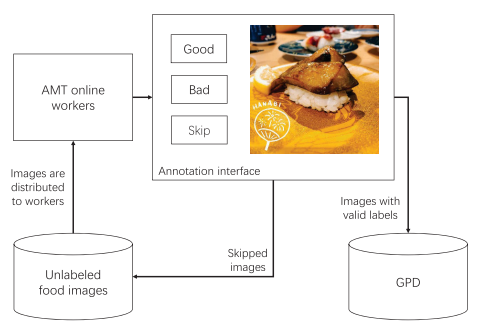
\includegraphics[scale=0.95]{images/pipeline.png}\caption{Schema tratto dal lavoro originale \cite{sheng2021learning} che illustra la pipeline della valutazione delle immagini del GPD da parte di 57 lavoratori del AMT (Amazon’s Mechanical Turk)}
\label{pipeline}
\end{figure}
	\item \textbf{Approvazione delle label da parte di otto fotografi esperti}, se almeno quattro di essi sono d'accordo con la label assegnata dagli utenti allora essa viene mantenuta, altrimenti la label è considerata ambigua e l'immagine viene eliminata.
\end{enumerate}
Le immagini verranno poi divise in modo randomico in:
\begin{itemize}
  \item \textbf{Training set}: 21600 immagini, di cui 
  \begin{itemize}
  \item 11779 positive
  \item 9821 negative
  \end{itemize}
  \item \textbf{Test set}: 10912 immagini, di cui
  \begin{itemize}
  \item 1309 positive
  \item 1091 negative
  \end{itemize}
\end{itemize}

\section{Test e risultati}
Nel lavoro originale \cite{sheng2021learning}, sono state provate varie combinazioni di feature e classificatore SVM (Support Vector Machine) con risultati di accuratezza sul test set abbastanza bassi, come è visibile nella prima parte della Tabella \ref{tabella_GPD}. In particolare le combinazioni sono le seguenti:
\begin{itemize}
\item \textbf{SVM e colore.} Il colore è una caratteristica molto significativa quando si parla di estetica, in questo caso il colore è stato codificato come un istogramma con 128 bin per i canali RGB. Inoltre i valori sono stati normalizzati rispetto alla media e alla varianza come segue:
\begin{equation} 
\label{normalizzazione}
x^{'}=\frac{x-\mu}{\sigma}
\end{equation}
In particolare $\mu$ indica la media, $\sigma$ indica la varianza e $x^{'}$ indica il valore $x$ a cui è stata applicata la normalizzazione.
\item \textbf{SVM e feature GIST.} Queste feature sono di tipo globale, in particolare viene estratto un array di feature con lunghezza pari a 512 partendo da una immagine a livelli di grigio di dimensione pari a 256x256. 
Anche in questo caso i valori sono stati normalizzati rispetto alla media e alla varianza come indicato al punto precedente in Formula ({\ref{normalizzazione}}).
\item \textbf{SVM e feature VGG.} Viene estratto un array di feature con lunghezza pari a 4096 dal penultimo layer di una rete VGG-16. In questo caso sono stati usati tre diversi modelli con contenuto semantico differente: VGG-objects, VGG-scenes e VGG-foods.
\end{itemize}
% cross entropy loss https://towardsdatascience.com/cross-entropy-loss-function-f38c4ec8643e
L'accuratezza cresce utilizzando delle reti neurali convoluzionali supervisionate, inizializzate con il dataset ImageNet \cite{deng2009imagenet} e utilizzando la cross-entropy per minimizzare la perdita e ottimizzare il modello. Nel training vengono utilizzate immagini scalate rispetto al lato più corto, tagliate e specchiate orizzontalmente in modo casuale al fine di aumentare il dataset disponibile.

\begin{table}[H]
\centering
\begin{tabular}{| c  c  c |}
\hline
Solution & Training Set & Test Set \\ [0.5ex]
\hline
%\textbf{SVM classifier} &  &  \\ [0.5ex]
\multicolumn{3}{|c|}{\textbf{SVM classifier}} \\ [0.5ex]
\hline
SVM + color & 72.4 & 63.3 \\
SVM + GIST & 78.1 & 64.4 \\
SVM + VGG-object & 90.8 & 74.7 \\
SVM + VGG-scenes & 86.8 & 72.4 \\
SVM + VGG-foods & 90.4 & 74.1 \\
\hline
%\textbf{Vanilla CNNs} &  &  \\ [0.5ex]
\multicolumn{3}{|c|}{\textbf{Vanilla CNNs}} \\ [0.5ex]
\hline
AlexNet & 89.1 & 88.6 \\
VGG-16 & 90.6 & 87.2 \\
InceptionV2 & 94.0 & 90.1 \\
ResNet-18 & 93.3 & 89.7 \\
\hline
%\textbf{CNNs for aesthethic assessment} &  &  \\ [0.5ex]
\multicolumn{3}{|c|}{\textbf{CNNs for aesthetic assessment}} \\ [0.5ex]
\hline
MP\ped{ada}\cite{sheng2018attention} & 94.6 & 90.4 \\
\hline
%\textbf{ResNet-18 with regularization} &  &  \\ [0.5ex]
\multicolumn{3}{|c|}{\textbf{ResNet-18 with regularization}} \\ [0.5ex]
\hline
ResNet-18 + aug & 93.6 & 89.9 \\
ResNet-18 + LSR\cite{szegedy2016rethinking} & 95.6 & 90.2 \\
ResNet-18 + $\sigma$\ped{T}\cite{hinton2015distilling} & 94.1 & 89.4 \\
ResNet-18 + ASR\cite{sheng2021learning} & 95.0 & 90.7 \\[1ex]
\hline  
\end{tabular}
\caption{Livelli di accuratezza e risultati raggiunti nel lavoro originale \cite{sheng2021learning} sul training set e sul test set utilizzando diversi approcci: combinazioni del classificatore SVM con diverse feature, reti neurali e reti neurali combinate con metodi di regolarizzazione}
\label{tabella_GPD}
\end{table}

Dagli esperimenti è emerso che la dimensione del GPD è sufficiente per classificare in maniera binaria l'estetica dei cibi, senza ricorrere a tecniche complesse di aumento delle immagini del dataset, inoltre il metodo di regolarizzazione ASR (Adaptive Smoothing Regularization) appositamente sviluppato \cite{sheng2021learning} risulta il migliore per quanto riguarda la confidenzialità dei risultati.

Le migliori performance, come è visibile in Tabella \ref{tabella_GPD}, sono ottenute tramite l'utlizzo del GPD insieme alle reti neurali, in particolare con la ResNet-18 combinata con ASR.  Attraverso altri metodi di regolarizzazione è possibile ottenere risultati di accuratezza sul test set attorno al 90\%, anche se con ASR è possibile ottenere una maggiore flessibilità.
%%%%%%%%%%%%%%%
\begin{comment}
In particolare utilizzando la rete Resnet-18, eventualmente combinata con diversi metodi di regolarizzazione, si ottengono le performance migliori. 

Il risultato migliore sul test set è ottenibile tramite questa rete e il metodo ASR (Adaptive Smoothing Regularization) \cite{sheng2021learning}. 
L'utilità dei metodi di regolarizzazione è principalmente quella di prevenire l'overfitting e aumentare le possibilità di generalizzazione.


In Tabella \ref{tabella_GPD} è ben visibile che anche con altri metodi di regolarizzazione è possibile ottenere buoni risultati a livello di accuratezza sul test set, anche se il metodo ASR offre una maggior flessibilità.
\end{comment}
%%%%%%%%%%%%%%

Un altro risultato degno di nota è legato alla semantica degli oggetti, in questo caso del cibo, quando bisogna valutarne l'estetica in quanto è ben visibile in Tabella \ref{tabella_GPD} che utilizzando il classificatore SVM combinato con le feature appartenenti a VGG-scenes l'accuratezza, sia sul test set che sul training set, è minore rispetto a quando si utilizza VGG-object o VGG-foods e ciò evidenzia che la semantica degli oggetti è significativa quando si vuole condurre una analisi sull'estetica di essi. 

Nel lavoro originale \cite{sheng2021learning}, a seguito di un ulteriore esperimento con 825 fotografie nuove sono state tratte alcune conclusioni, in particolare 50 candidati selezionati per valutare le immagini hanno ottenuto risultati coerenti rispetto a quelli ottenuti a livello teorico e ciò è particolarmente significativo, in quanto un buon modello per la valutazione estetica deve avere buone capacità di generalizzazione. Inoltre è emerso che le reti neurali supervisionate e parzialmente riaddestrate con il GPD posseggono questa grande capacità di generalizzazione, ciò porta a dimostrare la grandezza e l'importanza dei risultati ottenuti con l'uso del Gourmet Photography Dataset. 

Un'ulteriore evidenza significativa è che la valutazione estetica delle fotografie etichettate come negative è stata, in accordo con i risultati ottenuti, molto più semplice rispetto a quella delle immagini etichettate come positive, poiché gli utenti erano maggiormente in accordo tra loro e questo è il motivo che sta alla base del fatto che il GPD è sbilanciato con un maggior numero di immagini positive rispetto a quelle negative.



%Dagli esperimenti è emerso che è stato più semplice valutare le immagini etichettate come negative rispetto a quelle positive, poiché gli utenti erano maggiormente in accordo tra loro e per questo il GPD è sbilanciato con un maggior numero di immagini positive rispetto a quelle negative.



\chapter{Dataset proposto}
\label{new_dataset}
\section{Motivazione e composizione}
Per creare questo nuovo dataset sono state raccolte 146 nuove immagini, di cui 85 scattate da un fotografo professionista e 61 scattate da utenti non professionisti. É stato poi estrapolato da esse un sottoinsieme di 100 immagini, rispettivamente 50 professionali e 50 amatoriali, per poterle usare per valutare la capacità di generalizzazione della rete neurale che verrà usata successivamente.

Il motivo per cui si è scelto di proporre un nuovo dataset è stato quello di conoscere le prestazioni ottenute con la rete neurale, precedentemente utilizzata con il test set estratto dal GPD, e un nuovo set di immagini che la rete non avesse mai visto. Una particolarità evidente di questo dataset è il fatto che sia composto sia da fotografie professionali che da fotografie amatoriali, questo perché si è scelto di investigare il tema dell'estetica cercando di capire se la modalità di acquisizione e la tecnica fotografica possano influenzarne la percezione.

Le fotografie professionali sono state scattate nel corso degli anni da un fotografo professionista con macchine fotografiche Canon e principalmente con una lente a lunghezza focale fissa (50mm, 85mm o 100mm), che in questo caso permette di mettere a fuoco il soggetto e ottenere un effetto sfocato nel background, inoltre sono state precedentemente selezionate e contengono enhancement in quanto sono state scattate per menù e social network di ristoranti ed eventi perciò sono state necessarie queste operazioni prima di consegnarle agli utilizzatori finali.

Le fotografie amatoriali provengono da viaggi ed esperienze personali, sono state scattate principalmente da me in prima persona con iPhone 8 e iPhone 12 Pro oppure, in minima parte, da amici e non contengono enhancement di alcun tipo.

\section{Assegnamento delle groundtruth}
Inizialmente si pensava che le fotografie professionali fossero esteticamente belle, mentre quelle scattate dagli utenti non lo fossero, ma per confermare questa ipotesi è stato richiesto l'intervento di 41 utenti che valutassero le immagini in modo tale da ottenere le vere e proprie groundtruth, le quali potevano coincidere o meno con quelle ipotizzate inizialmente.
%Al fine di assegnare le label di groundtruth alle immagini del nuovo dataset,

\begin{comment}
\begin{figure}[H]
\centering
% scale= 0.72
% scale= 0.69
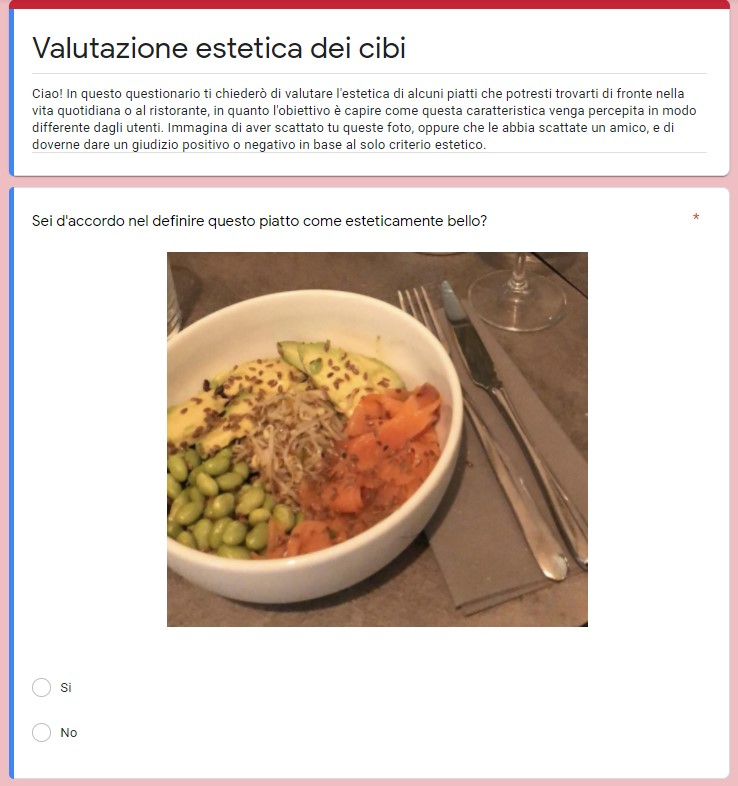
\includegraphics[scale= 0.69]{images/domanda questionario1.jpg}
\caption{Esempio di una delle domande del questionario che è servito per far valutare a 41 utenti le immagini del dataset proposto e ottenere le label di groundtruth}
\label{questionario1}
\end{figure}
\end{comment}

% inserimento Mock
\begin{figure}[H]
\centering
% scale=0.27
\includegraphics[scale=0.25]{images/mockup/Mockup_Q1.png}
\quad
\includegraphics[scale=0.25]{images/mockup/Mockup_D2Q1.png}
\quad
\caption{Esempio di una delle domande del questionario che è servito per far valutare a 41 utenti le immagini del dataset proposto e ottenere le label di groundtruth}
\label{questionario1}
\end{figure}

Prendendo ispirazione dallo stato dell'arte e da altri lavori sull'estetica \cite{sheng2021learning},  è stato creato un questionario all'interno del quale gli utenti hanno votato se, in base alla loro opinione e alla loro percezione dell'estetica, i piatti potevano essere considerati esteticamente belli o meno e, quindi, appartenere alla classe positiva o negativa. In base a questi voti sono state assegnate le label, in particolare per ogni immagine I$_i$ la corrispondente label binaria \^y$_{i}$ è data dalla maggioranza dei voti relativi a quella specifica immagine. Un esempio di una domanda del questionario è visibile in Figura \ref{questionario1}.

Di seguito, in Figura \ref{negativeNew}, sono riportate tutte le 27 immagini del dataset che  sono risultate avere una groundtruth negativa, mentre in Figura \ref{positiveNew} sono riportate tutte le 73 immagini che hanno groundtruth positiva. Si noti che nonostante si sia partiti da 50 immagini professionali e 50 amatoriali alla fine la numerosità di immagini con groundtruth negativa è minore di quella con groundtruth positiva, in quanto gli utenti hanno valutato positivamente anche alcune fotografie non professionali, ipoteticamente non concentrandosi sulla fotografia in sé bensì sul cibo stesso e pensando se quello specifico cibo fosse di loro gradimento. In minima parte ci sono stati anche casi in cui fotografie professionali sono state valutate negativamente.

% INSERIMENTO DI TUTTE LE IMMAGINI DEL DATASET
% negative
\begin{figure}[H]
\centering
\includegraphics[height=35mm]{images/new dataset/negative/negative (1).jpg}
\quad
\includegraphics[height=35mm]{images/new dataset/negative/negative (2).jpg}
\quad
\vspace{5mm}
\includegraphics[height=35mm]{images/new dataset/negative/negative (3).jpg}
\quad
\includegraphics[height=35mm]{images/new dataset/negative/negative (4).jpg}
\quad
\vspace{5mm}
\includegraphics[height=35mm]{images/new dataset/negative/negative (5).jpg}
\quad
\includegraphics[height=35mm]{images/new dataset/negative/negative (6).jpg}
\quad
\includegraphics[height=35mm]{images/new dataset/negative/negative (7).jpg}
\quad
\vspace{5mm}
\includegraphics[height=35mm]{images/new dataset/negative/negative (8).jpg}
\quad
\includegraphics[height=35mm]{images/new dataset/negative/negative (9).jpg}
\quad
\end{figure}

% vanno splittate per gestire la fine della pagina 
\begin{figure}[H]
\centering
\includegraphics[height=35mm]{images/new dataset/negative/negative (10).jpg}
\quad
\includegraphics[height=35mm]{images/new dataset/negative/negative (11).jpg}
\quad
\includegraphics[height=35mm]{images/new dataset/negative/negative (12).jpg}
\quad
\includegraphics[height=35mm]{images/new dataset/negative/negative (13).jpg}
\quad
\vspace{5mm}

\includegraphics[height=35mm]{images/new dataset/negative/negative (14).jpg}
\quad
\includegraphics[height=35mm]{images/new dataset/negative/negative (15).jpg}
\quad
\includegraphics[height=35mm]{images/new dataset/negative/negative (16).jpg}
\quad
\vspace{5mm}
\includegraphics[height=35mm]{images/new dataset/negative/negative (17).jpg}
\quad
%%
\includegraphics[height=35mm]{images/new dataset/negative/negative (18).jpg}
\quad
\includegraphics[height=35mm]{images/new dataset/negative/negative (19).jpg}
\quad
\includegraphics[height=35mm]{images/new dataset/negative/negative (20).jpg}
\quad 
\vspace{5mm}
\includegraphics[height=35mm]{images/new dataset/negative/negative (21).jpg}
\quad
\includegraphics[height=35mm]{images/new dataset/negative/negative (22).jpg}
\quad
\vspace{5mm}
\includegraphics[height=35mm]{images/new dataset/negative/negative (23).jpg}
\quad
\includegraphics[height=35mm]{images/new dataset/negative/negative (24).jpg}
\quad
%\vspace{5mm}
\includegraphics[height=35mm]{images/new dataset/negative/negative (25).jpg}
\quad
\includegraphics[height=35mm]{images/new dataset/negative/negative (26).jpg}
\quad
\includegraphics[height=35mm]{images/new dataset/negative/negative (27).jpg}
\caption{Immagini del dataset a cui è stata assegnata una groundtruth negativa tramite i voti degli utenti}
\label{negativeNew}
\end{figure}

% positive
\begin{figure}[H]
\centering
\includegraphics[height=35mm]{images/new dataset/positive/positive (1).jpg}
\quad
\includegraphics[height=35mm]{images/new dataset/positive/positive (2).jpg}\quad
\includegraphics[height=35mm]{images/new dataset/positive/positive (3).jpg}\quad
\vspace{5mm}
\includegraphics[height=35mm]{images/new dataset/positive/positive (4).jpg}\quad
\includegraphics[height=35mm]{images/new dataset/positive/positive (5).jpg}\quad
\includegraphics[height=35mm]{images/new dataset/positive/positive (6).jpg}\quad
\vspace{5mm}
\includegraphics[height=35mm]{images/new dataset/positive/positive (7).jpg}\quad
\includegraphics[height=35mm]{images/new dataset/positive/positive (8).jpg}\quad
\vspace{5mm}
\includegraphics[height=35mm]{images/new dataset/positive/positive (9).jpg}\quad
\includegraphics[height=35mm]{images/new dataset/positive/positive (10).jpg}\quad
\vspace{5mm}
\includegraphics[height=35mm]{images/new dataset/positive/positive (11).jpg}\quad
\includegraphics[height=35mm]{images/new dataset/positive/positive (12).jpg}\quad
\includegraphics[height=35mm]{images/new dataset/positive/positive (13).jpg}\quad
\vspace{5mm}
\includegraphics[height=35mm]{images/new dataset/positive/positive (14).jpg}\quad
\includegraphics[height=35mm]{images/new dataset/positive/positive (15).jpg}\quad
\end{figure}

\begin{figure}[H]
\centering
\includegraphics[height=35mm]{images/new dataset/positive/positive (16).jpg}\quad
\includegraphics[height=35mm]{images/new dataset/positive/positive (17).jpg}\quad
\vspace{5mm}
\includegraphics[height=35mm]{images/new dataset/positive/positive (18).jpg}\quad
\includegraphics[height=35mm]{images/new dataset/positive/positive (19).jpg}\quad
\includegraphics[height=35mm]{images/new dataset/positive/positive (20).jpg}\quad
\vspace{5mm}
\includegraphics[height=35mm]{images/new dataset/positive/positive (21).jpg}
\quad
\includegraphics[height=35mm]{images/new dataset/positive/positive (22).jpg}\quad
\includegraphics[height=35mm]{images/new dataset/positive/positive (23).jpg}\quad
\vspace{5mm}
\includegraphics[height=35mm]{images/new dataset/positive/positive (24).jpg}\quad
\includegraphics[height=35mm]{images/new dataset/positive/positive (25).jpg}\quad
\includegraphics[height=35mm]{images/new dataset/positive/positive (26).jpg}\quad
\vspace{5mm}
\includegraphics[height=35mm]{images/new dataset/positive/positive (27).jpg}\quad
\includegraphics[height=35mm]{images/new dataset/positive/positive (28).jpg}\quad
\includegraphics[height=35mm]{images/new dataset/positive/positive (29).jpg}\quad
\includegraphics[height=35mm]{images/new dataset/positive/positive (30).jpg}\quad
\includegraphics[height=35mm]{images/new dataset/positive/positive (31).jpg}\quad
\includegraphics[height=35mm]{images/new dataset/positive/positive (32).jpg}\quad
\includegraphics[height=35mm]{images/new dataset/positive/positive (33).jpg}\quad
\end{figure}

\begin{figure}[H]
\centering
\includegraphics[height=35mm]{images/new dataset/positive/positive (34).jpg}\quad
\includegraphics[height=35mm]{images/new dataset/positive/positive (35).jpg}
\quad
\includegraphics[height=35mm]{images/new dataset/positive/positive (36).jpg}\quad
\vspace{5mm}
\includegraphics[height=35mm]{images/new dataset/positive/positive (37).jpg}\quad
\includegraphics[height=35mm]{images/new dataset/positive/positive (38).jpg}\quad
\includegraphics[height=35mm]{images/new dataset/positive/positive (39).jpg}\quad
\vspace{5mm}
\includegraphics[height=35mm]{images/new dataset/positive/positive (40).jpg}\quad
\includegraphics[height=35mm]{images/new dataset/positive/positive (41).jpg}\quad
\includegraphics[height=35mm]{images/new dataset/positive/positive (42).jpg}\quad
\vspace{5mm}
\includegraphics[height=35mm]{images/new dataset/positive/positive (43).jpg}\quad
\includegraphics[height=35mm]{images/new dataset/positive/positive (44).jpg}\quad
\vspace{5mm}
\includegraphics[height=35mm]{images/new dataset/positive/positive (45).jpg}\quad
\includegraphics[height=35mm]{images/new dataset/positive/positive (46).jpg}\quad
\vspace{5mm}
\includegraphics[height=35mm]{images/new dataset/positive/positive (47).jpg}\quad
\end{figure}

\begin{figure}[H]
\centering
\includegraphics[height=35mm]{images/new dataset/positive/positive (48).jpg}\quad
\includegraphics[height=35mm]{images/new dataset/positive/positive (49).jpg}\quad
\vspace{5mm}
\includegraphics[height=35mm]{images/new dataset/positive/positive (50).jpg}\quad
\includegraphics[height=35mm]{images/new dataset/positive/positive (51).jpg}\quad
\includegraphics[height=35mm]{images/new dataset/positive/positive (52).jpg}\quad
\vspace{5mm}
\includegraphics[height=35mm]{images/new dataset/positive/positive (53).jpg}
\quad
\vspace{5mm}
\includegraphics[height=35mm]{images/new dataset/positive/positive (54).jpg}\quad
\includegraphics[height=35mm]{images/new dataset/positive/positive (55).jpg}\quad
\includegraphics[height=35mm]{images/new dataset/positive/positive (56).jpg}\quad
\vspace{5mm}
\includegraphics[height=35mm]{images/new dataset/positive/positive (57).jpg}\quad
\includegraphics[height=35mm]{images/new dataset/positive/positive (58).jpg}\quad
\includegraphics[height=35mm]{images/new dataset/positive/positive (59).jpg}\quad
\includegraphics[height=35mm]{images/new dataset/positive/positive (60).jpg}\quad
\end{figure}

\begin{figure}[H]
\centering
\includegraphics[height=35mm]{images/new dataset/positive/positive (61).jpg}\quad
\includegraphics[height=35mm]{images/new dataset/positive/positive (62).jpg}\quad
\vspace{5mm}
\includegraphics[height=35mm]{images/new dataset/positive/positive (63).jpg}\quad
\includegraphics[height=35mm]{images/new dataset/positive/positive (64).jpg}
\quad
\vspace{5mm}
\includegraphics[height=35mm]{images/new dataset/positive/positive (65).jpg}\quad
\includegraphics[height=35mm]{images/new dataset/positive/positive (66).jpg}\quad
\vspace{5mm}
\includegraphics[height=35mm]{images/new dataset/positive/positive (67).jpg}\quad
\includegraphics[height=35mm]{images/new dataset/positive/positive (68).jpg}\quad
\includegraphics[height=35mm]{images/new dataset/positive/positive (69).jpg}\quad
\vspace{5mm}
\includegraphics[height=35mm]{images/new dataset/positive/positive (70).jpg}\quad
\includegraphics[height=35mm]{images/new dataset/positive/positive (71).jpg}\quad
\includegraphics[height=35mm]{images/new dataset/positive/positive (73).jpeg}
\quad
\includegraphics[height=35mm]{images/new dataset/positive/positive (72).jpg}\quad
\caption{Immagini del dataset a cui è stata assegnata una groundtruth positiva tramite i voti degli utenti}
\label{positiveNew}
\end{figure}

Al fine di identificare cosa avesse portato gli utenti a fornire una determinata valutazione è stato creato un secondo questionario analogo al precedente, con la differenza che veniva richiesto loro di motivare il perché di ogni risposta fornita. Un esempio di domanda è riportato in Figura \ref{questionario2}.

% inserimento Mock
\begin{figure}[H]
\centering
% scale=0.27
\includegraphics[scale=0.25]{images/mockup/Mockup_Q2.png}
\quad
\includegraphics[scale=0.25]{images/mockup/Mockup_D2Q2.png}
\quad
\caption{Esempio di una delle domande del questionario che è servito per far valutare a 11 utenti le immagini del dataset proposto e a motivare il perché di tale valutazione al fine di comprendere su che aspetti dell'immagine si fossero focalizzati}
\label{questionario2}
\end{figure}

Il questionario è stato completato da un sottoinsieme di 11 utenti, dai quali è emerso che un cibo esteticamente bello deve essere ben disposto all'interno del piatto, deve essere appetitoso agli occhi di chi lo osserva e se i colori catturano l'attenzione è più probabile che venga valutato positivamente. Inoltre è stata confermata l'ipotesi precedente, ovvero che alcuni utenti in diversi casi hanno valutato positivamente una fotografia non concentrandosi sulla tecnica fotografica utilizzata, ma sul gusto del cibo stesso o sulla sua presentazione. 

Ad esempio un utente, per suo gusto personale, non ha apprezzato una fotografia di carne grigliata poiché ipoteticamente potrebbe essere vegetariano oppure semplicemente potrebbe non piacergli questo cibo in particolare.

In Figura \ref{esempioNeg} viene mostrata una immagine che ha ottenuto  11 voti negativi su 11, le principali motivazioni sono la scarsa accuratezza nella preparazione e composizione del piatto, il fatto che il cibo è già stato in parte mangiato e che si nota la scarsa qualità della fotografia in quanto essa è leggermente sfocata.

\begin{figure}[H]
\centering
% scale=0.18
\includegraphics[scale=0.20]{images/new dataset/negative/negative (11).jpg}
\caption{Esempio di una immagine che ha ottenuto solo voti negativi nel secondo questionario, principalmente a causa del fatto che il cibo non ha una composizione accurata, è già stato mangiato e la fotografia è leggermente sfocata}
\label{esempioNeg}
\end{figure}

In Figura \ref{esempioPos} viene mostrata una immagine che ha ottenuto 11 voti positivi su 11, essa risulta molto colorata e il contrasto cromatico tra i colori dei poke e il tavolo attira l'attenzione di chi osserva, inoltre la composizione della fotografia e del cibo stesso è molto curata e attenta.

\begin{figure}[H]
\centering
% scale=0.30
\includegraphics[scale=0.33]{images/new dataset/positive/positive (29).jpg}
\caption{Esempio di una immagine che ha ottenuto solo voti positivi nel secondo questionario, gli utenti si sono concentrati principalmente sui colori molto vivaci che formano un bel contrasto cromatico con il tavolo e sulla composizione accurata dei poke}
\label{esempioPos}
\end{figure}


\chapter{Metodologie per la classificazione}
\label{metodologie}

\section{Feature hand-crafted}
% \cite{spathis2016photo}
Dopo aver suddiviso le immagini del dataset GPD come già illustrato nel Capitolo~\ref{GPD} sono stati osservati i vari tipi di feature in letteratura, al fine di capire quali utilizzare. Le feature possono essere suddivise in 4 principali categorie \cite{spathis2016photo}:
\begin{enumerate}
\item \textbf{Feature relative al colore}, ad esempio combinazioni lineari dei tre canali degli spazi colore HSV o HSL oppure la media di essi. 
\item \textbf{Feature relative alla texture}, ad esempio lo studio degli edge, LBP (Local Binary Pattern), CEDD (Color and Edge Directivity Descriptor) o QHist ovvero l'istogramma dei canali RGB quantizzati a 16 livelli ciascuno.
\item \textbf{Feature relative alla composizione}, ad esempio lo studio del blur, delle linee tramite la trasformata di Hough, l'aspect ratio o la regola dei terzi.
\item \textbf{Feature relative al contenuto}, ovvero la ricerca di determinati oggetti o aree in una immagine, ad esempio un volto oppure la pelle.
\end{enumerate} 

\section{Un'ulteriore suddivisione delle immagini}
\label{divisione}
Dopo aver analizzato più a fondo i datastore, ovvero le strutture utilizzate in MATLAB \cite{MATLAB} per gestire i vari set di immagini, è stato scelto di lavorare con set bilanciati in modo da avere una probabilità equa per le due classi. 

In particolare le immagini sono state ulteriormente divise come segue:
\begin{itemize}
  \item \textbf{Set di Rigetto}: 2176 immagini positive che portavano le due classi ad essere sbilanciate, in particolare questo set di immagini non verrà più utilizzato nel proseguo del lavoro. Si avranno 21824 immagini in totale, ovvero la differenza tra il numero totale di immagini (24000) e il numero di immagini appartenenti a questo set.
\item \textbf{Training set}: 17678 immagini, ovvero il 90\% del 90\% del nuovo numero totale di immagini (21824). Si prende una prima volta il 90\% delle immagini poiché il restante 10\% sarà poi parte del Test set, successivamente se ne prende ancora il 90\% perché il restante 10\% sarà assegnato al Validation set. In particole le immagini del Training set saranno divise come segue:
  \begin{itemize}
  \item 8839 positive
  \item 8839 negative
  \end{itemize}
  \item \textbf{Test set}: 2182 immagini, ovvero il restante 10\% dopo la prima divisione, di cui
  \begin{itemize}
  \item 1091 positive
  \item 1091 negative
  \end{itemize}
  \item \textbf{Validation set}: 1964 immagini, ovvero il restante 10\% dopo la seconda divisione del Training set, di cui
  \begin{itemize}
  \item 982 positive
  \item 982 negative
  \end{itemize}
\end{itemize}

\section{Feature estratte da una rete neurale}

Per cercare di migliorare i risultati ottenuti con le feature hand-crafted si è scelto di utilizzare una rete neurale da cui estrarre delle feature di più alto livello e passarle a un classificatore, in questo caso un SVM. La rete scelta per questa fase è stata la ResNet-18 poiché era quella più utilizzata in altri esperimenti \cite{sheng2021learning} presi come riferimento e che allo stesso tempo otteneva anche buoni risultati.
% eventualmente grafico resnet18

È stato ipotizzato anche l'uso della VGG-16 ma è stata preferita la ResNet-18 in quanto dopo alcuni test si è notato che era più lenta nel riaddestramento e anche meno utilizzata negli esperimenti presi come riferimento.

Quando bisogna estrarre le feature da una rete neurale è necessario specificare il layer della rete da cui estrarle, in questo caso con la rete ResNet-18 sono stati fatti due test, uno con il layer pool5 e uno con il layer res3b\_relu. Essi si trovano in parti diverse della rete, infatti il layer pool5 si trova alla fine della rete, mentre il layer res3b\_relu si trova più o meno a metà di essa.


\section{Uso di una rete neurale per l'intera classificazione}

\subsection{Prima implementazione}
Al fine di incrementare ulteriormente l'accuratezza ottenuta nelle fasi precedenti del lavoro si è scelto di utilizzare una ResNet-18 pre-addestrata su cui svolgere una operazione di Fine Tuning, ovvero una parziale modifica della rete al fine di adattarla per svolgere un nuovo task. In particolare in questa fase sono stati modificati il Fully Connected layer e il Classification Output layer in modo tale che lavorino con due classi e restituiscano in output solo una di esse. 

Nella fase di riaddestramento della rete è stato necessario scegliere se compiere delle operazioni di aumento del dataset disponibile in particolare, traendo ispirazione dal lavoro originale \cite{sheng2021learning}, si è scelto di compiere scaling sia lungo l'asse x che lungo l'asse y, traslazione e riflessione rispetto all'asse x in maniera casuale al fine di aumentare il numero di immagini disponibili. 

É stato necessario anche impostare alcuni parametri tra cui il numero massimo di epoche, ovvero il massimo numero di cicli di training, la dimensione del batch, ovvero un parametro che definisce il numero di campioni con cui lavorare prima di aggiornare i parametri interni al modello, e il tasso di apprendimento iniziale della rete neurale.


\subsection{Early Stopping}

Durante la fase di riaddestramento della rete si è osservato che, dopo un determinato periodo di tempo, il grafico dell'accuratezza tendeva a rimanere costante e ciò significa che la rete non stava più apprendendo nulla dai dati forniti ad essa. Per questo motivo si è scelto di implementare l'Early Stopping o stop anticipato, il quale permette di fermare il processo di training se l'accuratezza non migliora oppure se la funzione Loss peggiora per un certo numero di epoche consecutive. 

In questo caso si è scelto di implementare lo stop basandosi sull'accuratezza, ad esempio se si sceglie di fermare l'addestramento dopo due epoche dove l'accuratezza non si incrementa di fatto si otterranno almeno tre epoche di training, in quanto la rete controllerà se l'accuratezza si è mantenuta minore o uguale a quella della prima epoca nelle due epoche successive e, in caso affermativo, fermerà il processo.

Lo stop anticipato può permettere un risparmio di tempo e risorse durante il Fine Tuning, ma ciò dipende da come si impostano i parametri iniziali e dal numero di epoche dopo le quali si sceglie di fermare il processo. 

É importante segnalare che il processo di Early Stopping potrebbe non essere sempre vantaggioso in quanto è possibile ottenere anche casistiche nelle quali, nonostante lo si utilizzi, vengano comunque compiute tutte le epoche di training perché l'accuratezza risulterà sempre in crescita e quindi la rete non fermerà il training in anticipo, poiché si cerca sempre di ottenere il miglior risultato possibile.
 
% TO DO: Nel Capitolo dei Risultati va inserita una sezione per riportare l'accuratezza ottenuta sul mio Dataset, con eventuali problematiche legate agli exif
 
\section{Valutazione del dataset proposto}
\label{valutazione}
Per tutto il resto del lavoro è stata utilizzata la rete ResNet-18 riaddestrata con Early Stopping che ha ottenuto migliori risultati sia sul test set che sul validation set, ovvero quella con Initial Learn Rate pari a 0.0005, stop anticipato dopo due epoche delle sei epoche possibili e dimensione del batch pari a dieci.

Con questa rete sono state valutate le immagini del dataset proposto, prestando attenzione al fatto che in MATLAB alcune immagini erano visualizzate ruotate di 90 gradi a causa di metadati contenuti all'interno delle immagini stesse, per cui è stato necessario un processing mirato su alcune immagini al fine di avere tutto il dataset visualizzato correttamente. 

Inizialmente, come già specificato, si era pensato di utilizzare come groundtruth delle label ricavate secondo il criterio che una fotografia professionale fosse esteticamente bella, e quindi avesse label positiva, mentre una fotografia scattata da un utente non lo fosse, e quindi avesse label negativa. Ciò è parso poco sensato, in quanto osservando le immagini del dataset proposto riportate nel Capitolo~\ref{new_dataset} in Figura \ref{negativeNew} e Figura \ref{positiveNew} si può notare che alcune immagini non professionali sono state comunque etichettate come positive dagli utenti nel questionario a loro sottoposto e viceversa, ciò sta a significare che non sempre c'è una corrispondenza tra tecnica nello scatto ed estetica di esso, anche se generalmente molte fotografie professionali sono percepite come esteticamente belle poiché utilizzano colori, contrasti e tecniche che gli utenti apprezzano molto.

A seguito di questa considerazione si è quindi scelto di utilizzare come groundtruth per la valutazione le label risultanti dal questionario, in quanto esse catturano in maniera particolare la percezione dell'estetica del dataset proposto da parte di un particolare gruppo di 41 utenti che sono stati presi come campione per questo esperimento. In particolare le immagini saranno distribuite nelle due classi come segue:
\begin{itemize}
\item \textbf{Groundtruth appartenente alla classe positiva}: 73 immagini
\item \textbf{Groundtruth appartenente alla classe negativa}: 27 immagini
\end{itemize}


\section{Grad-CAM per capire le predizioni}

Al fine di comprendere quali porzioni di un'immagine vengano maggiormente prese in considerazione dalla rete per determinare la label predetta è stata utilizzata la tecnica del Gradient-weighted Class Activation Mapping (Grad-CAM) \cite{selvaraju2017grad}, la quale evidenzia in rosso le aree più significative e in blu quelle meno significative per la predizione della rete fornendo una visualizzazione facilmente interpretabile da chi la osserva ed essendo applicabile a molte famiglie di reti neurali convoluzionali. 

In particolare la tecnica in questione utilizza il gradiente relativo al concetto che si è scelto come target nell'immagine, il quale entra negli ultimi layer convoluzionali, con l'obiettivo di produrre una mappa che mostri le aree più significative e quelle meno significative relative al tema scelto. Si utilizzano proprio questi layer poiché le feature convoluzionali conservano informazioni spaziali, le quali vengono perse all'interno del Fully Connected layer e quindi gli ultimi layer convoluzionali prima di esso permettono di conciliare una buona semantica con queste informazioni che sono molto significative se, come in questo caso, si vuole analizzare quale area dell'immagine è più rilevante per la classificazione di essa da parte di una rete neurale.

Un esempio di applicazione della tecnica Grad-CAM ad una immagine è riportato in Figura \ref{gradcam_gen}.

\begin{figure}[H]
\centering
\includegraphics[height=50mm]{images/gradcam_generica.jpg}
\caption{Esempio di una immagine a cui è stata applicata la tecnica Grad-CAM focalizzandosi su due differenti classi di oggetti, in questo caso prima sulla classe "Gatto" e poi sulla classe "Cane", il quale è stato tratto dal lavoro originale sulla tecnica Grad-CAM \cite{selvaraju2017grad}}
\label{gradcam_gen}
\end{figure}

%%%%%
\begin{comment}
\begin{figure}[H]
\centering
\includegraphics[height=45mm]{images/gradcam1.jpg}
\quad
\includegraphics[height=45mm]{images/gradcam23.jpg}
\quad
\includegraphics[height=45mm]{images/gradcam14.jpg}
\quad
\caption{Esempi di immagini a cui è stata applicata la tecnica Grad-CAM dove la rete ha predetto correttamente una label negativa}
\label{gradcam_neg}
\end{figure}

\begin{figure}[H]
\centering
\includegraphics[height=45mm]{images/gradcam53.jpg}
\quad
\includegraphics[height=45mm]{images/gradcam85.jpg}
\quad
\includegraphics[height=45mm]{images/gradcam28.jpg}
\quad
\caption{Esempi di immagini a cui è stata applicata la tecnica Grad-CAM dove la rete ha predetto correttamente una label positiva}
\label{gradcam_pos}
\end{figure}
\end{comment}
%%%%%

Osservando le immagini ricavate con la tecnica appena illustrata applicata alle immagini del dataset proposto sembrava potesse esserci una correlazione tra la predizione della rete e la porzione di immagine che veniva considerata più significativa, ovvero quella colorata di rosso.

Al fine di avere una misura oggettiva che potesse aiutare a comprendere se ci fosse o meno questa correlazione è stato necessario compiere alcuni passaggi preliminari:

\begin{itemize}
\item \textbf{Creazione di maschere binarie}, le quali avessero in bianco il cibo e in nero il background, un esempio è riportato in Figura \ref{mask}. Esse sono state realizzate con l'ausilio di Photoshop, ma sarebbe andato bene anche un altro editor di immagini.
\begin{figure}[H]
\centering
\includegraphics[height=45mm]{images/Resized53.jpg}
\quad
\includegraphics[height=45mm]{images/Resized85.jpg}
\quad
\includegraphics[height=45mm]{images/Resized1.jpg}
\quad
\caption{Esempi di maschere binarie dei cibi, le quali mostrano in bianco il cibo e in nero il background}
\label{mask}
\end{figure}
\item \textbf{Calcolo del rapporto tra area della maschera e area totale dell'immagine}, tale rapporto è stato espresso in percentuale ed è indicato con $A_{m}$.
\item \textbf{Calcolo del rapporto tra energia che ricade nella maschera ed energia totale}, dove con energia si intende l'intensità della mappa Grad-CAM per ogni pixel. Questo passaggio è stato fatto ponendo attenzione a normalizzare i valori delle mappe Grad-CAM rispetto al valore minimo e massimo, in modo tale da ottenere valori tra zero e uno, come segue:
\begin{equation} 
\label{normalizzazione_minmax}
x^{'}=\frac{x-min}{max-min}
\end{equation}
In particolare anche questo rapporto è stato espresso in percentuale per comodità e viene indicato con $E_{m}$.
\item \textbf{Calcolo dell'indicatore di concentrazione dell'energia}, ovvero calcolo del seguente rapporto:
\begin{equation} 
\label{indicatore}
C=\frac{E_{m}}{A_{m}}
\end{equation}
Tale valore per definizione sarà un valore decimale e non una percentuale, poiché è definito come rapporto tra due percentuali. Si è scelto di mantenerlo in questa forma per comodità nel visualizzare grafici che lo rappresentassero al fine di correlarlo alle predizioni della rete. 
\end{itemize}
\chapter{Risultati ottenuti}
\label{risultati}

\section{Risultati ottenuti sul dataset GPD}
\subsection{Feature hand-crafted}

Per prima cosa sono stati analizzati i risultati ottenuti con le feature hand-crafted, ovvero le più semplici, i quali sono riportati in Tabella \ref{tabella_handcrafted}.

\begin{table}[H]
\resizebox{\columnwidth}{!}{
\centering
\begin{tabular}{| c | c | c | c |}
\hline
Feature & Classificatore & Training Set & Test Set\\ [0.5ex]
\hline
LBP & SVM & 0.7276 & 0.6987 \\
CEDD & SVM & 0.6788 & 0.6529 \\
QHist & SVM & 0.6931 & 0.6904 \\
LBP, CEDD, QHist & SVM & 0.6766 & 0.6667 \\
Media H, Media S, Intensità & SVM & 0.5813 & 0.6075 \\
Pleasure, Arousal, Dominance & SVM & 0.5688 & 0.5850 \\
Media H, Media S, LBP & SVM & 0.7357 & 0.7446 \\
Media H, Media S, CEDD & SVM & 0.6772 & 0.6854 \\
Pleasure, Arousal, Dominance, LBP & SVM & 0.7277 & 0.7383 \\
Pleasure, Arousal, Dominance, CEDD & SVM & 0.6821 & 0.6867 \\
\hline
\end{tabular}}
\caption{Livelli di accuratezza ottenuti sul training set e sul test set utilizzando diverse combinazioni di feature e il classificatore SVM}
\label{tabella_handcrafted}
\end{table}

In questo caso sono state usate principalmente feature legate al colore e alla texture e il miglior risultato sul test set è stato ottenuto combinando la media di canali H e S insieme a LBP, quindi unendo descrittori legati al colore e alla texture. Inoltre in tabella sono stati riportati i risultati su test set e su training set, i quali sono stati divisi come illustrato nel Capitolo~\ref{GPD}, per poter fare un immediato confronto con i risultati ottenuti nel lavoro originale \cite{sheng2021learning}, i quali sono stati riportati in Tabella \ref{tabella_GPD}. 

\subsection{Feature estratte da una rete neurale}

Di seguito, in Tabella \ref{tabella_estrazione}, sono riportati i risultati ottenuti con feature estratte da due layer differenti di una rete ResNet-18 e, in particolare, non c'è una grande differenza di accuratezza estraendo le feature da un layer che si trova più in profondità all'interno della rete come il layer pool5 rispetto a uno che si trova meno in profondità come il layer res3b\_relu, anzi l'accuratezza è leggermente più elevata nel secondo caso.

Di seguito, così come negli studi successivi, verranno riportati i livelli di accuratezza ottenuti sul test set e sul validation set come spiegato precedentemente in Sezione~\ref{divisione} del Capitolo~\ref{metodologie} al fine di utilizzare dei dataset che avessero una numerosità equa di immagini in ognuna delle due classi.

\begin{table}[H]
\centering
\begin{tabular}{| c | c | c | c | c |}
\hline
Rete & Classificatore & Layer & Test Set & Validation Set\\ [0.5ex]
\hline
ResNet-18 & SVM & pool5 & 0.8350 & 0.8452 \\
ResNet-18 & SVM & res3b\_relu & 0.8391 & 0.8478 \\
\hline
\end{tabular}
\caption{Livelli di accuratezza ottenuti sul validation set e sul test set utilizzando il classificatore SVM con delle feature estratte da due diversi layer della rete ResNet-18. Nel primo caso le feature sono state estratte dal layer pool5, il quale si trova alla fine della rete, mentre nel secondo caso dal layer res3b\_relu, il quale si trova a metà della rete}
\label{tabella_estrazione}
\end{table}

\subsection{Uso delle reti neurali per l'intera classificazione}

Quando ci si affida completamente all'uso di una rete neurale è necessario differenziare quando si utilizzi la tecnica dell'Early Stopping rispetto a quando non la si utilizzi, ciò porta nella maggior parte dei casi a uno spreco di tempo e risorse poiché vengono eseguite tutte le epoche del riaddestramento della rete anche se, come già anticipato nel Capitolo~\ref{metodologie}, non è detto che l'uso del Fine Tuning combinato con l'Early Stopping diminuisca il numero di epoche effettivamente svolte in quanto ciò dipende da come vengono impostati i vari parametri e da come cresce l'accuratezza durante l'esecuzione.

I risultati ottenuti senza stop anticipato sono riportati in Tabella \ref{tabella_rete1}, mentre quelli relativi all'esecuzione con Early Stopping sono riportati in Tabella \ref{tabella_rete2}.

\begin{table}[H]
\resizebox{\columnwidth}{!}{
\centering
\begin{tabular}{| c | c | c | c | c | c |}
\hline
Rete & Test Set & Validation Set & Initial Learn Rate &	Epochs & Batch Size \\  [0.5ex]
\hline
ResNet-18 & 0.8882 & 0.89 & 0.0003 & 6 & 10	\\
ResNet-18 & 0.8996 & 0.8905 & 0.0005 & 6 & 10	\\
ResNet-18 & 0.8731 & 0.8849 & 0.00003 & 6 & 10	\\
ResNet-18 & 0.8520 & 0.8493 & 0.00001 & 6 & 10	\\
ResNet-18 & 0.8744 & 0.8829 & 0.0003 & 8 & 10	\\
\hline
\end{tabular}}
\caption{Livelli di accuratezza ottenuti sul validation set e sul test set utilizzando una procedura di Fine Tuning su una rete ResNet-18. Sono stati riportati anche i parametri utilizzati per inizializzare il numero di epoche, la dimensione del batch e il tasso di apprendimento iniziale della rete} 
\label{tabella_rete1}
\end{table}


\begin{table}[H] 
\resizebox{\columnwidth}{!}{
\centering
\begin{tabular}{| c | c | c | c | c | c | c |}
\hline
Rete & Test Set & Validation Set & Initial Learn Rate &	Epochs & Batch Size & Early Stopping \\  [0.5ex]
\hline
ResNet-18 & 0.9051 & 0.9043 & 0.0005 & 6 & 10 & 2 epoche \\	
ResNet-18 & 0.9015 & 0.8946 & 0.0003 & 6 & 10 & 2 epoche \\
ResNet-18 & 0.8579 & 0.8569 & 0.00003 & 6 & 10 & 1 epoca \\
ResNet-18 & 0.8437 & 0.8462 & 0.00001 & 6 & 10 & 1 epoca \\
% Fa tutte e 6 le epoche
ResNet-18 & 0.8799 & 0.8997 & 0.0003 & 8 & 10 & 2 epoche \\
\hline
\end{tabular}}
\caption{Livelli di accuratezza ottenuti sul validation set e sul test set utilizzando una procedura di Fine Tuning su una rete ResNet-18 con Early Stopping dopo una o due epoche, a seconda di quale  valore portasse a un maggior risparmio di tempo, anche se nel caso di stop anticipato dopo una sola epoca con Initial Learn Rate pari a 0.00001 non c'è stato alcun miglioramento in quanto sono state eseguite comunque tutte le epoche del training. Sono stati riportati anche i parametri utilizzati per inizializzare il numero di epoche, la dimensione del batch e il tasso di apprendimento iniziale della rete} 
\label{tabella_rete2}
\end{table}

\section{Risultati ottenuti sul dataset proposto}

\subsection{Analisi delle groundtruth}

Osservando la distribuzione delle groundtruth delle immagini del dataset proposto, la quale è riportata in Sezione~\ref{valutazione} del Capitolo~\ref{metodologie}, si osserva che gli utenti hanno valutato positivamente 73 immagini del dataset e negativamente le restanti 27. Questo risultato è sbilanciato verso la classe positiva, nonostante inizialmente siano state utilizzate 50 immagini professionali e 50 scattate da utenti comuni non professionisti, ciò mostra come la percezione dell'estetica dei cibi, ma anche in qualsiasi altro ambito, non è strettamente legata alla tecnica fotografica utilizzata o alla struttura della fotografia bensì entrano in gioco anche altri fattori soggettivi, tra cui il background culturale, le abitudini alimentari e gli specifici gusti del sottoinsieme di utenti che sono stati chiamati a valutare le immagini del dataset proposto.

\subsection{Uso di una rete neurale adattata}

Come già anticipato nel Capitolo~\ref{metodologie} per valutare l'estetica nel dataset proposto è stata utilizzata principalmente la rete neurale che ha ottenuto i migliori risultati ovvero, come riportato in Tabella \ref{tabella_rete2}, quella che ha un Initial Learn Rate pari a 0.0005 e che utilizza l'Early Stopping dopo due epoche nelle quali l'accuratezza non migliora.

Utilizzando come groundtruth le label ottenute dal questionario che è stato sottoposto a 41 utenti, la cui distribuzione è stata analizzata precedentemente, e la rete precedentemente citata è stata ottenuta una accuratezza del 72\%.

In questa fase è stata molto significativa l'analisi degli errori compiuti dalla rete e la successiva analisi delle immagini generate con la tecnica Grad-CAM \cite{selvaraju2017grad}, in particolare si evince che la rete ha classificato 17 immagini come falsi negativi, ovvero è stata predetta la label negativa mentre la groundtruth era positiva, e 11 falsi positivi, ovvero è stata predetta la label positiva mentre la groundtruth era negativa. 

Di seguito, in Figura \ref{gradcam_neg} e in Figura \ref{gradcam_pos}, sono riportate alcune delle immagini del dataset proposto a cui è stata applicata la tecnica Grad-CAM e dove la rete non ha compiuto errori di classificazione.

\begin{figure}[H]
\centering
\includegraphics[height=45mm]{images/gradcam1.jpg}
\quad
\includegraphics[height=45mm]{images/gradcam23.jpg}
\quad
\includegraphics[height=45mm]{images/gradcam14.jpg}
\quad
\caption{Esempi di immagini a cui è stata applicata la tecnica Grad-CAM dove la rete ha predetto correttamente una label negativa}
\label{gradcam_neg}
\end{figure}

\begin{figure}[H]
\centering
\includegraphics[height=45mm]{images/gradcam53.jpg}
\quad
\includegraphics[height=45mm]{images/gradcam85.jpg}
\quad
\includegraphics[height=45mm]{images/gradcam28.jpg}
\quad
\caption{Esempi di immagini a cui è stata applicata la tecnica Grad-CAM dove la rete ha predetto correttamente una label positiva}
\label{gradcam_pos}
\end{figure}

In Figura \ref{FalseNeg} è riportato un esempio di immagine appartenente ai falsi negativi, mentre in Figura \ref{FalsePos} è invece riportato un esempio di immagine appartenente ai falsi positivi. Entrambe le immagini di esempio sono riportate insieme alle rispettive Grad-CAM al fine di poter mostrare eventuali differenze nella posizione delle aree più significative, in rosso, e di quelle meno significative, in blu, rispetto al cibo. Questa tematica verrà approfondita nella Sezione~\ref{analisiGradCAM} insieme ad altre ipotesi scaturite dall'analisi delle Grad-CAM, le quali hanno portato a investigare la correlazione tra l'indicatore di concentrazione dell'energia e le predizioni della rete.

\begin{figure}[H]
\centering
\includegraphics[height=45mm]{images/falseNegImg.jpg}
\quad
\includegraphics[height=45mm]{images/falseNegCAM.jpg}
\quad
\caption{Esempio di una immagine per la quale la rete ha predetto la label negativa mentre la groundtruth era positiva, per cui essa rientra tra gli errori e in particolare tra i falsi negativi. A destra viene riportata anche la rispettiva Grad-CAM, dalla quale si nota che le aree che la rete ha considerato più significative per la predizione della label non sono quelle del cibo, bensì appartengono al piatto e allo sfondo}
\label{FalseNeg}
\end{figure}

\begin{figure}[H]
\centering
\includegraphics[height=45mm]{images/falsePosImg.jpg}
\quad
\includegraphics[height=45mm]{images/falsePosCAM.jpg}
\quad
\caption{Esempio di una immagine per la quale la rete ha predetto la label positiva mentre la groundtruth era negativa, per cui essa rientra tra gli errori e in particolare tra i falsi positivi. A destra viene riportata anche la rispettiva Grad-CAM, dalla quale si nota che le aree che la rete ha considerato più significative per la predizione della label sono effettivamente quelle del cibo e non altre parti dell'immagine}
\label{FalsePos}
\end{figure}

\subsection{Analisi delle Grad-CAM}
\label{analisiGradCAM}
Come già evidenziato in precedenza l'analisi delle immagini ricavate con la tecnica Grad-CAM è fondamentale al fine di individuare cosa la rete consideri significativo per l'effettiva predizione della label ed eventualmente per individuare nessi causali tra queste aree, considerate più significative per la predizione, e gli errori compiuti. Infatti osservando le Grad-CAM sembrava che quando l'area più significativa veniva individuata al di fuori del cibo la rete predicesse la label negativa, perciò si è scelto di indagare più a fondo sfruttando l'indicatore di concentrazione dell'energia. 

Per confermare quest'ultima ipotesi è stato costruito un grafico, visibile in Figura \ref{graficoRappPred}, nel quale l'indicatore di concentrazione, riportato sull'asse x e calcolato come espresso in Formula (\ref{indicatore}), viene correlato alle predizioni della rete, riportate sull'asse y. Al fine di rappresentare le label in maniera numerica si è scelto di far corrispondere alla label negativa il valore -1 e alla label positiva il valore 1, in modo tale che la distinzione nel grafico fosse evidente, inoltre si è scelto un grafico di tipo Scatter Plot perché visivamente mostra molto bene la distribuzione dei punti e perché esso dava la possibilità di inserire sugli assi cartesiani due diverse variabili, che in questo caso sono le predizioni e l'indicatore di concentrazione C.

Osservando il grafico è ben visibile che gli elementi della classe positiva sono molto più numerosi di quelli della classe negativa, le immagini sono infatti classificate dalla rete come segue:
% eventualmente togliere \newpage, in questo caso l'ho messo per far si che non si "spezzasse" l'elenco puntato
\newpage
\begin{itemize}
\item \textbf{Classe positiva}: 67 elementi
\item \textbf{Classe negativa}: 33 elementi
\end{itemize}

É molto interessante la distribuzione vera e propria di questi elementi, rappresentati nello Scatter Plot come dei pallini, poiché si nota che al di sopra di un certo valore di soglia, che potrebbe essere individuato attorno al valore 1 sull'asse delle x, è possibile separare le due classi commettendo pochi errori. Questa distribuzione mostra una correlazione tra le variabili inserite sugli assi cartesiani così come era stato ipotizzato, al crescere dell'indicatore di concentrazione dell'energia all'interno dell'area corrispondente al cibo cresce la probabilità che venga predetta la label positiva, in particolare man mano che aumenta la concentrazione si osserva che le predizioni diventano tutte appartenenti alla classe positiva.

\begin{figure}[H]
\centering
\includegraphics[height=87mm]{images/graficoRappPred.png}
\caption{Grafico che rappresenta sull'asse delle x l'indicatore di concentrazione per ognuna delle immagini del dataset proposto, mentre sull'asse delle y rappresenta le label predette, in particolare il valore -1 indica la label negativa mentre il valore 1 indica la label positiva}
\label{graficoRappPred}
\end{figure}

Questo risultato è davvero significativo poiché conferma l'ipotesi fatta in precedenza, mostrando che quando la Grad-CAM si focalizza correttamente sulla porzione di immagine occupata dal cibo si avrà che la concentrazione di energia in quell'area sarà elevata e, quindi, sarà più probabile che la rete predica una label positiva.

Il risultato va però contestualizzato, in determinati casi entrano in gioco fattori di gusto personale degli utenti e fattori legati alla semantica dell'immagine analizzata che possono essere imprevedibili per la rete neurale in quanto, come già sottolineato, l'estetica è una caratteristica puramente soggettiva e che può variare nel tempo, in quanto un utente potrebbe valutare positivamente un cibo e, in un momento successivo, valutare lo stesso cibo in maniera opposta poiché il suo background culturale e il suo bagaglio di esperienze potrebbero avergli fatto modificare la sua personale concezione di bellezza.






\chapter{Conclusioni e sviluppi futuri}
\label{sviluppi}

\begin{comment}
\begin{itemize}
\item riportare parte dell'intro, spiegando l'obiettivo 
\item immagini negative più semplici da valutare, su quelle positive c'è più discordanza tra gli utenti
\item si conferma che l'estetica è una caratteristica molto soggettiva e piuttosto complessa da descrivere con dei modelli
\item ipotetici sviluppi futuri: possibile ampliamento del mio dataset e ampliamento dei 41 utenti, i quali dovranno anche motivare le risposte in modo più esaustivo possibile, in modo tale da avere più opinioni così come è stato fatto nel Paper \cite{sheng2021learning}
\end{itemize}
\end{comment}

La relazione si è basata sul lavoro svolto durante l'esperienza di stage presso l'Ateneo, il cui obiettivo è stato in primo luogo l'analisi di un dataset di immagini di cibo già esistente. Il dataset in questione è il Gourmet Photography Dataset o GPD \cite{sheng2021learning}, il quale contiene 24000 immagini di cibi con le relative label, le quali possono appartenere alla classe positiva o alla classe negativa a seconda della valutazione estetica della singola immagine.

Si è scelto di utilizzare diverse feature con grado di astrazione e difficoltà crescente, partendo dalle feature hand-crafted e arrivando fino all'uso di una rete neurale, opportunamente modificata e adattata, per l'intera classificazione delle immagini del dataset. Lo sviluppo di codice per l'intero lavoro è stato in linguaggio MATLAB \cite{MATLAB}.

Successivamente è stato proposto un dataset creato ad hoc per sperimentare l'utilizzo di una rete neurale appositamente adattata e osservare i risultati ottenuti, confrontandoli con quelli conseguiti con il dataset già esistente. In particolare ci si è poi concentrati sullo studio di ciò che la rete considerava più importante per determinare la label predetta, ovvero una tematica molto interessante e che permette di capire il ragionamento alla base delle valutazioni compiute dalla rete neurale.

A seguito delle analisi svolte durante l'esperienza di stage sul dataset proposto si è osservato che gli utenti tendono a valutare positivamente le immagini, anche se queste fotografie non sono professionali, concentrandosi soprattutto sul cibo e non sulla tecnica fotografica. Inoltre, come già si ipotizzava dopo aver studiato altri lavori \cite{sheng2021learning} già esistenti sul tema dell'estetica dei cibi, si è confermato che l'utilizzo delle reti neurali ottiene migliori performance rispetto all'utilizzo di descrittori più semplici combinati con un classificatore.

Per quanto riguarda i possibili sviluppi di questa ricerca si potrebbe ipotizzare un sostanziale ampliamento del dataset proposto, portandone la numerosità delle immagini a livelli pari di altri dataset famosi come il GPD, e un ampliamento della popolazione che, tramite il primo dei due questionari, ha fornito le valutazioni delle immagini per determinare le groundtruth utilizzate.  Di pari passo con questo ampliamento verrebbe ampliata anche la popolazione che è stata richiamata per completare un secondo questionario, il cui obiettivo era raccogliere le motivazioni degli utenti a seguito della valutazione di ogni singola immagine.
L'incremento del numero di utenti coinvolti potrebbe essere particolarmente significativo, in quanto maggiore è il numero di persone che valutano le immagini più sarà possibile osservare il comportamento di esse ed eventualmente modificare la raccolta delle groundtruth o la valutazione delle immagini stesse.

Un possibile sviluppo più a lungo termine potrebbe essere l'integrazione di questo studio in un'applicazione che, data una fotografia di cibo, ne dia una valutazione estetica e fornisca delle motivazioni relative ad essa, in modo tale che ristoranti e chiunque fotografi il cibo possa comprendere se, di fronte a un'immagine valutata negativamente, il problema sia relativo alla fotografia in sé oppure sia legato alla presentazione del cibo. Ciò potrebbe essere utile nell'ottica di creare fotografie non professionali per i social network di un ristorante, un bar oppure semplicemente per chi ama scattare fotografie a ciò che mangia per pubblicarle. Scattare velocemente una foto ed eventualmente applicare qualche filtro di color correction direttamente dallo smartphone, caricarla nell'app e ottenere la valutazione potrebbe essere un processo rapido e semplice prima della pubblicazione di tale fotografia e potrebbe aiutare soprattutto chi usa i social network a livello commerciale per comprendere se l'immagine finale può essere adatta al proprio pubblico su un determinato social network, dato che online gli utenti vengono attirati da fotografie colorate, con contrasti, giochi di luce particolari e, nel caso del cibo, che siano ben strutturate per mostrare qualcosa di appetitoso.


%\cleardoublepage
%\phantomsection
%\addcontentsline{toc}{chapter}{\bibname}
%\printbibliography

\newpage
\printbibheading[heading=bibintoc, title={Riferimenti}]
\printbibliography[nottype=online,heading=subbibintoc,title={Bibliografia}]
\printbibliography[type=online,heading=subbibintoc,title={Siti}]
\end{document}